\documentclass[11pt]{article}
\usepackage{fullpage}
\usepackage{graphicx}
\usepackage{enumitem}
\usepackage{float}
\usepackage{placeins}
\usepackage{url}
\setlength{\parindent}{0pt}
\setlength{\parskip}{5pt plus 2pt minus 1pt}

\title{CS63 Spring 2024\\Enhancing AI Performance in 2048: Genetic Algorithms and\\ Direct Policy Learning}
\author{Zixi Gao, Xiaoya Yuan}
\date{}

\begin{document}

\maketitle

\section{Introduction}

% Your paper should be 4-6 pages long.  In this section you should give
% a broad introduction to your project.  Assume that you are writing to
% an audience that is familiar with AI, but may not know the details of
% the particular technique that you are using.  You should give an
% overview of the approach being explored, and how you applied it to a
% particular problem. 

In this project, we explore the application of artificial intelligence techniques to play the classic game of 2048, a puzzle game that challenges players to slide numbered tiles on a grid to combine them into increasingly higher powers of two. The goal of the game is to create a 2048 tile and to continue until no further tiles can be combined. To tackle this, previous papers have introduced minimax and expectimax with alpha-beta pruning or Monte-Carlo Tree-Search and Averaged Depth-Limited Search and produced promising results (Rodgers \& Levine, 2014; Feske, Aashir, \& Rohan, 2014). In our work, we experimented with two different methodologies: Genetic Algorithms (GA) and Direct Policy Learning via GA.

Initially, we employed a GA where each chromosome represents a sequence of moves. Through the processes of selection, crossover, and mutation, we evolved these chromosomes to identify the sequence that maximizes the game score, ideally aiming to create a tile with a value of 512. While this approach yielded satisfactory results, it had limitations. The GA operated without knowledge of the game state during evolution, essentially resulting in random chromosome combinations.

To address this, we shifted to Direct Policy Learning through Genetic Algorithms. In this approach, a neural network takes a flattened array of the board's 16 tiles as input and outputs weights for the four possible move directions. This method employs GA to evolve the weights of the neural network to predict the optimal move based on the game state, representing a more informed and strategic approach to playing 2048.

\section{Methods}

% In this section you should explain the details about your project.

% For example, if your project is based on a Kaggle competition, this should include
% describing the data set used (number of patterns, number of features,
% description of features, any preprocessing that was necessary) and its
% source.

% You should provide all of the parameter settings used (such as
% learning rate, etc.).  You should also provide details about how the
% system was trained, and how you determined when to end training.

% Details about how to test and run your \emph{code} should NOT be given in the
% paper, but should instead be described in the README file in the lab
% directory. 
\subsection{Implementation of 2048 Game}

Our implementation of the 2048 game in Python utilizes a two-dimensional list to represent the 4x4 board, with each sublist corresponding to a row on the game board, essential for effectively simulating the game's grid dynamics. The gameplay is facilitated by several helper functions responsible for transposing the board, compressing and merging cells, and randomly inserting a new tile with a 2 tile if game doesn't end. The game initiates with two tiles of 2 placed on the grid and progresses until there are no valid moves lfet or until a 2048 tile is formed. Unlike web or app versions, our implementation lacks graphical interfaces and operates purely through console outputs that can display the board's state, focusing on the functional aspects crucial for subsequent analysis using genetic algorithms and direct policy learning.

\subsection{Genetic Algorithm}
In our genetic algorithm approach for the 2048 game, we employ chromosomes that encode sequences of game moves, represented by the directions ‘w’, ‘s’, ‘a’, and ‘d’ for up, down, left, and right, respectively. Fitness evaluation takes place once a game sequence concludes, either when all encoded moves are executed or no further moves can be made on the board. Our fitness function calculates the total game score based on the values of tiles merged during gameplay. The formation of higher-value tiles significantly boosts the fitness, exemplified by the creation of a 512 tile. This occurs when two 256 tiles merge, resulting in a total score over 4096 points, demonstrating the game's exponential scoring system. This scoring approach aligns the fitness of a chromosome with its effectiveness at navigating and optimizing gameplay on the 2048 board.

In our GA framework:

\begin{itemize}[leftmargin=*]
  \item \textbf{Selection} is implemented using a roulette wheel strategy, where the probability of a chromosome being selected for reproduction correlates with its fitness score. Individuals with higher fitness are more likely to be chosen.
  \item \textbf{Crossover} is implemented through an one-point method, where segments of two parent chromosomes are swapped at a randomly chosen position, controlled by a crossover probability (\texttt{pCrossover}). 
  \item \textbf{Mutation} involves randomly altering the direction of move within a chromosome with a mutation probability (\texttt{pMutation}). Specifically, the mutated move will always be different from the original, ensuring diversity within the gene pool. 
\end{itemize}

Key adjustable parameters include \texttt{pCrossover}, \texttt{pMutation}, \texttt{pop\_size} (population size), \texttt{length} (length of the chromosome), and number of evolutionary generations. These parameters were tuned to maximize training outcomes.

\subsection{Direct Policy Learning via Genetic Algorithms}
Transitioning from our GA framework, we employ a neural network-based Direct Policy Learning that also utilizes a form of GA, with the same notions of selection, mutation, and crossover. Contrary to previous model where each chromosome represents the moves per game, this model encodes each chromosome as a set of weights for a neural network, learning the policy for move selection based on the game state. The neural network features 16 inputs which corresponds to the flattened array of the 16 tiles of the game board, each represented by an integer. The output of the neural network represents the four possible directional moves (‘w’, ‘s’, ‘a’, ‘d’) that the AI can make at any step in the game. The size of the hidden layer(s) is configurable, allowing us to tune the network for higher game scores. The sets of weights of the neural network will be generated at random initially, and get evolved during each generation of GA. 

We developed the \texttt{Env2048} environment, based on Gym's standard \texttt{Env}, to facilitate game state initialization and step simulation. This environment can reset to the initial state of 2048 and simulate moves given the current state and selected action, returning 1) the new state, 2) the reward of the move, and 3) the done status indicating the end of each step.

The fitness of each chromosome is evaluated by the total score as AI plays the game to completion or until no further moves are available. The moves are dictated by the neural network’s output, which strategically selects actions to maximize the score. The population of chromosomes is iteratively evolved over a given number of generations, with continuous adjustments to the neural network's weights to enhance the performance of playing 2048.

\section{Results \& Discussion}

% In this section you should show and analyze the results.  Measure the
% performance of your system, and if possible compare your performance
% to other implementations. Use tables and figures to illustrate the
% results.  You should also discuss what sorts of conclusions can be drawn from
% these results; what did you learn, what are the important takeaways for a
% reader, etc.

% Even if your project is not as successful as you'd hoped, you still
% need to show and discuss results.  This section is one of the key parts of any
% scientific paper.  Be sure to provide adequate information so that the
% reader can evaluate the outcomes of your experiments. 
\subsection{Genetic Algorithm}
The performance of our genetic algorithm (GA) was evaluated through multiple generations with different parameters. Figure \ref{fig:fitness} illustrates the result of the GA training. It shows the evolution of fitness across 70 generations, demonstrating significant variation in performance with a peak fitness score of 4576 points. This peak corresponds to the successful formation of a 512 tile as shown in Figure \ref{fig:4576endgame}.

\begin{figure}[ht]
\centering
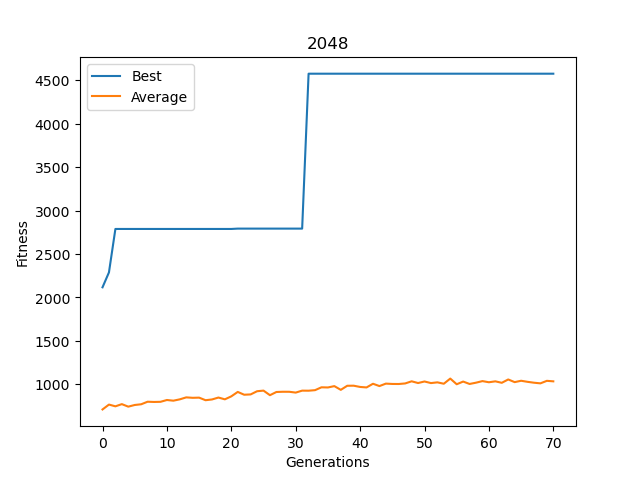
\includegraphics[width=0.8\textwidth]{4576.png}
\caption{Best GA training result with evolution over 70 generations and a peak in performance with a fitness of 4576 points.}
\label{fig:fitness}
\end{figure}

\begin{figure}[ht]
\centering
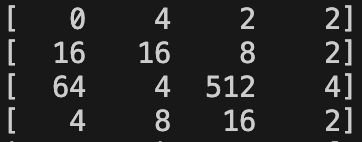
\includegraphics[width=0.4\textwidth]{4576board.png}
\caption{The game board's end state of GA training corresponding to the highest fitness achieved of 4576 points. Tiles with larger values are piled at the center of the board.}
\label{fig:4576endgame}
\end{figure}

\newpage
The parameters leading to the highest fitness were carefully selected:
\begin{itemize}
    \item \textbf{Crossover Probability (\texttt{pCrossover})}: 0.05
    \item \textbf{Mutation Probability (\texttt{pMutation})}: 0.1
    \item \textbf{Chromosome Length (\texttt{length})}: 330
    \item \textbf{Population Size (\texttt{pop\_size})}: 300
    \item \textbf{Number of Generations}: 70
\end{itemize}

The choice of a chromosome length of 330 moves was based on theoretical calculations, suggesting approximately 300 moves are required to achieve a 512 tile. This length ensures a balance between computational efficiency and the potential for achieving high-value tiles. The low crossover probability (0.05) was set to maintain the sequential integrity of moves, as random swapping could disrupt the build-up necessary for game success. Conversely, a relatively high mutation rate (0.1) was employed to introduce variation and adaptability, helping the algorithm avoid local maxima by potentially triggering advantageous tile placements.

As illustrated in Figure \ref{fig:fitness}, the fitness levels consistently remained around 2700 across numerous generations, then abruptly increased to exceed 4500. This dramatic increase is directly linked to the formation of a 512 tile, underscoring the GA's reliance on probabilistic outcomes to generate effective move sequences. While achieving this high fitness level is a significant success of GA training, the rarity of forming a 512 tile illustrates the limitations of the GA in consistently learning and optimizing game strategies.

Building on this, the average fitness of the population showed a gradual increase, suggesting some degree of learning or optimization despite the probabilistic nature of the GA. However, further analysis of the board's end state revealed that high-value tiles often appeared in non-optimal positions, unlike strategic human play which typically positions high-value tiles in the corners. This limitation of traditional GA methods, which tend to generate high-value tiles through random combinations of moves rather than strategic planning, prompted us to refine our approach.

\newpage
\subsection{Direct Policy Learning via Genetic Algorithms}
Motivated by observations of GA, we explored the implementation of Direct Policy Learning within the same GA framework for the 2048 game. This new strategy focuses more on the adaptability and efficiency of learning mechanisms by evolving the weights of the neural network to predict a move. As depicted in Figure \ref{fig:results}, the Direct Policy Learning approach exhibits a consistent increase in learning performance, peaking at a fitness score of 2402 points at the 50th generation. This peak, corresponding to the creation of a 256 tile as shown in Figure \ref{fig:2402endgame}, illustrates how the approach gradually optimizes its tile-merging strategy to achieve higher scores, showcasing a significant advancement from the earlier GA-only strategies.

\begin{figure}[ht]
\centering
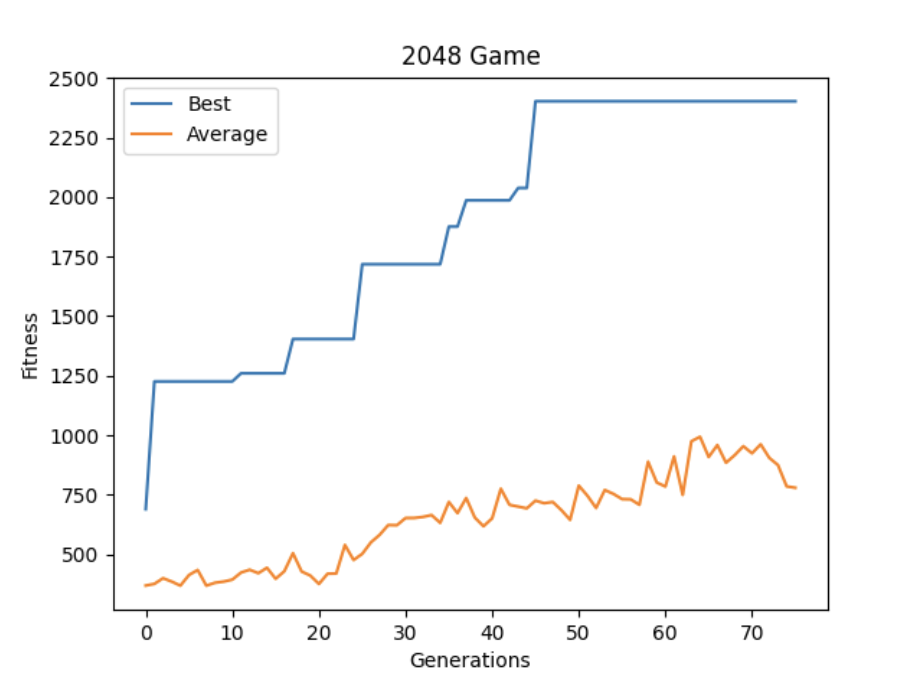
\includegraphics[width=0.8\textwidth]{2402.png}
\caption{Fitness progression over 70 generations with Direct Policy Learning GA, illustrating steady improvement and peak fitness achievement.}
\label{fig:results}
\end{figure}

\FloatBarrier

\begin{figure}[ht]
\centering
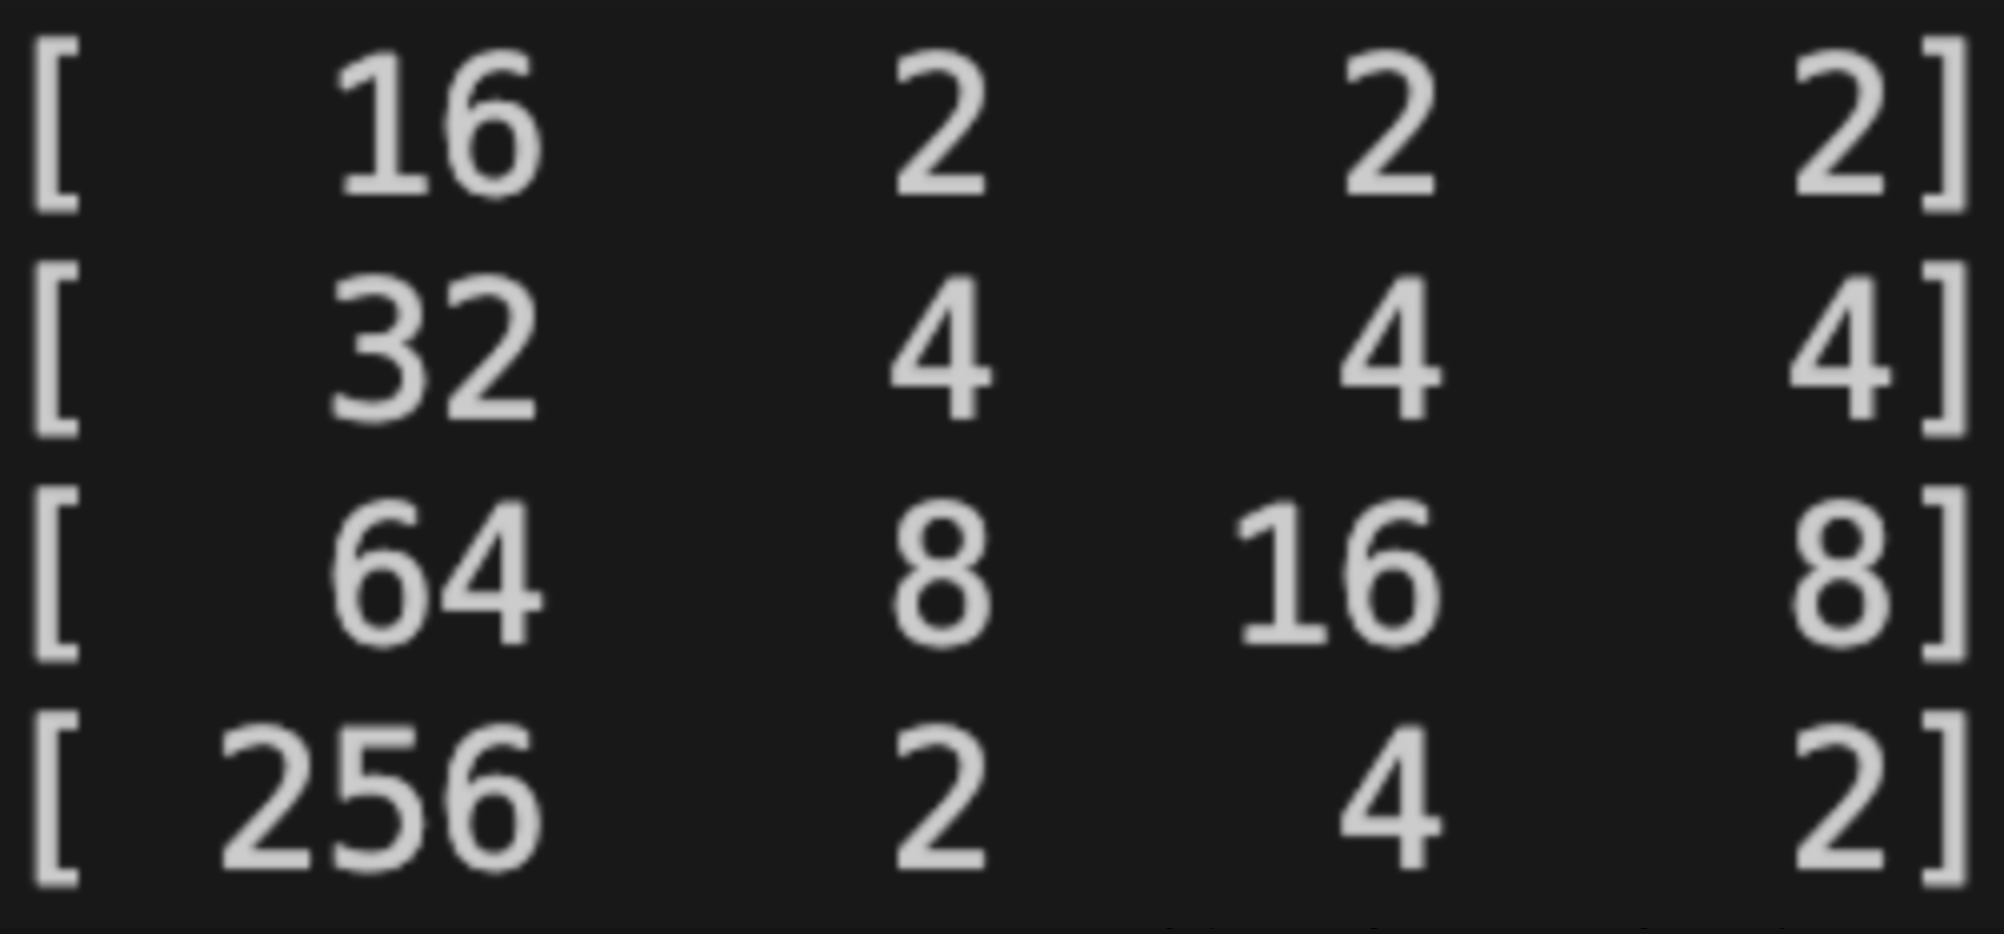
\includegraphics[width=0.4\textwidth]{2402board.png}
\caption{The game board after the Direct Policy Learning training. It corresponds to the highest fitness achieved of 2402 points. Tiles with larger values are piled to the bottom left corner.}
\label{fig:2402endgame}
\end{figure}

\textbf{Key Parameters and Their Impact:}
\begin{itemize}
    \item \textbf{Size of Hidden Layer (\texttt{hid\_sizes)}:} [6]. The optimal configuration was a single hidden layer with 6 nodes instead of multiple layers. This simpler structure avoided the vanishing gradient problem often seen with deeper networks and proved sufficient for capturing the necessary strategic depth required for 2048.
    \item \textbf{Crossover Probability (\texttt{pCrossover}):} 0.8, this high rate guaranteed sufficient exploration of the genetic space, encouraging diverse genetic combinations that potentially led to innovative strategies.
    \item \textbf{Mutation Probability (\texttt{pMutation}):} 0.75, it promotes a high level of variation within the gene pool, crucial for preventing premature convergence to local maximum.
    \item \textbf{Steps:} 250, which denotes the number of moves the AI was allowed to make per game, providing a substantial number of actions to learn from while ensuring the training sessions remained manageable.
\end{itemize}

Throughout the training process with Direct Policy Learning via GA, it was observed that while the AI demonstrated an ability to achieve moderately high tile values, it frequently failed to position similar tiles adjacently in a manner that maximizes merging opportunities. This is evident from the end-game board state shown in Figure \ref{fig:endgame}. 

\begin{figure}[ht]
\centering
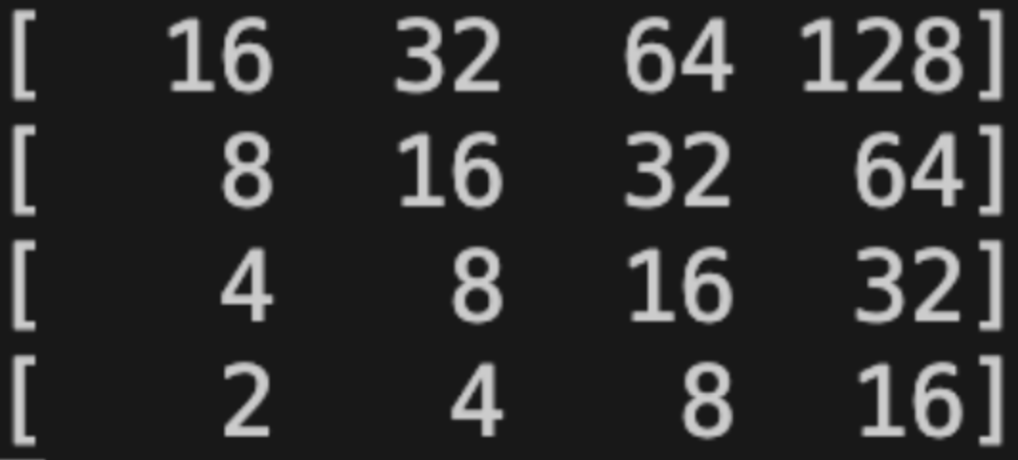
\includegraphics[width=0.4\textwidth]{figure3.png}
\caption{Example of a common game board at the end of a training session achieved by the Direct Policy Learning via GA. It highlights a significant limitation in strategy formation.}
\label{fig:endgame}
\end{figure}

We made an attempt to address this issue by adjusting the reward function to favor board states with adjacent tiles of same value. The modification has led to improvements, allowing the AI to occasionally generate a 256 tile, as opposed to frequently becoming trapped in less optimal states like those commonly seen in Figure \ref{fig:endgame}.

The behavioral pattern as seen in Figure \ref{fig:endgame}, however, shows a critical limitation of the Direct Policy Learning approach. While the AI successfully learns the strategy to pile higher values in the upper right corner, it often fails to recognize when to deviate from this strategy and execute opposite moves that would enable merging of these tiles. This limitation arises because the AI does not analyze each game state individually but instead applies a consistent set of weights in the neural network throughout the game, making only minor adjustments. As a result, while the neural network is adept at optimizing for immediate tile movements and accumulating high-value tiles in one corner, it is not capable for long-term decision-making necessary for forming tiles of 1024 and beyond. The Direct Policy Learning approach using GA is good at optimizing a set of actions based on what it has seen during training but can struggle with strategy shifts that were not sufficiently emphasized during the learning phase.

\section{Conclusions}

% In our exploration of the 2048 game using genetic algorithms (GA) and direct policy learning via GA, both models demonstrated distinct advantages and limitations. The GA model has yielded fruitful results with generating a 512 tile but failed to account for the game state. This oversight led to situations where no more tiles could be added or merged before running all the steps, prematurely terminating the game. The lack of perception of game states in the GA model demonstrates its limitations in predicting and avoiding end-game scenarios.

% Conversely, the neural GA exhibited behavior similar to human players, who arrange the highest-value tiles into the corner to prompt easier merging. The game board exhibits a strategic "staircase" formation where tiles are arranged in descending order of their values. This pattern highlighted the neural GA's ability to learn complex strategies involving tile placement and movement during the 2048 game and is thought to avoid the limitations in the GA model. However, the model struggled to navigate out of local minima, where directional changes are required to deviate from the corner-stacking strategy. This indicates a need for further refinement in its fitness evaluation functions, as high levels of mutation and crossover were insufficient to overcome these challenges. This observation aligns with findings from another paper employing artificial neural networks (ANN) in the 2048 game (Feske, Aashir, \& Rohan, 2014).

Our exploration of the 2048 game using genetic algorithms (GA) and direct policy learning via GA has revealed distinct advantages and shortcomings of each model. The GA model successfully generated a 512 tile, yet it often failed to consider the overall game state, leading to premature game terminations where no further tiles could be merged or added. This limitation in the GA model's ability to foresee and navigate end-game scenarios reflects its deficiency in strategic depth. In contrast, the neural GA more closely mimicked human strategic behavior, notably arranging higher-value tiles into corners to facilitate easier merging. The game board often exhibited a strategic "staircase" formation, demonstrating the neural GA's capacity to learn complex tile placement and movement strategies. However, this model sometimes became stuck in local maxima, particularly when a change in direction was necessary to break away from a corner-stacking strategy. This suggests that further refinement of the fitness evaluation functions is necessary, as high mutation and crossover rates alone were not enough to avoid these strategic pitfalls.

Building on insights and previous findings that models trained on abstract game state qualities outperform those trained on raw data (Feske, Aashir, \& Rohan, 2014), we plan to refine our fitness function to focus more on specific, quantifiable metrics such as the number of empty tiles, the presence of adjacent tiles of the same value, and the degree of monotonicity across the board. To further enhance our direct policy learning approach, we are exploring alternative neural network architectures, including convolutional neural networks (CNNs), which are adept at processing two-dimensional spatial data like the 2048 game grid. Additionally, using a framework such as Keras to implement advanced activation functions like ReLU may optimize tile merging strategies, addressing the neural GA's current limitations and improving its strategic capabilities.


\section{Acknowledgements}

We are grateful to the academic and online sources for their valuable insights into AI strategies for the 2048 game. Our 2048 game is adapted from the logic.py from geeksforgeeks. The discussions on Stack Overflow and the Rodgers, P., \& Levine, J. paper inspired our focus on developing AI algorithms for the 2048 game. The insights from Gajjar et al. have inspired us to change our fitness functions and improve our algorithms. We thank Professor Ben Mitchell for his instruction about different AI algorithms and Professor Lisa Meeden for her strategic advice on employing neural genetic algorithms to overcome limitations in our GA model. We would like to thank our peers Zhengfei Li, Ziji Wang, and Zehua You who provided essential feedback during the peer review process. Additionally, we used ChatGPT for LaTeX formatting assistance. We would like to thank all these contributions who were instrumental throughout our project.

\newpage
\section{References}

Aashir, G., Rohan, K., \& Feske, J. (2014). 2048: Learning to Play 2048. Retrieved from http://www.joelfeske.com/2048.html

\vspace{10pt}

GeeksforGeeks. (2023, January 23). 2048 game in Python. https://www.geeksforgeeks.org/2048-game-in-python/ 

\vspace{10pt}

Rodgers, P., \& Levine, J. (2014). An investigation into 2048 AI strategies. In \textit{Proceedings of the 2014 IEEE Conference on Computational Intelligence and Games (CIG)}. IEEE. Retrieved from https://doi.org/10.1109/CIG.2014.6932920

\end{document}